\section{Ren mechanistic diagnosis (arXiv:2601.10679)}
\label{sec:ren}

Following Ren et al., we probe whether post-grokking degradation reflects \emph{latent guessing} (fixed-point violation, ACT-depth sensitivity) versus \emph{Nanda-style cleanup} (FVE collapse under weight decay while accuracy stays high).

\paragraph{Protocol.}
For each TRM seed we run Ren probes at three checkpoints: final, grokking, and best-FVE.
Metrics: fixed-point violation rate, ACT-depth accuracy curve, critical ACT-step grokking step, latent PCA at ``$=$''.

\paragraph{Full TRM.}
Full TRM exhibits Ren-style failure modes: non-zero fixed-point violation and accuracy drop as max ACT steps increase (Figure~\ref{fig:ren_act}).
Latent trajectories show non-monotonic refinement (Figure~\ref{fig:pca_ren}).

\paragraph{TRM minimal (null test).}
Minimal TRM uses a single ACT step; ACT-depth ablation collapses to that step.
When fixed-point violation and depth sensitivity are near zero, we classify post-grokking FVE loss as \textbf{Nanda cleanup}, not Ren guessing (Table~\ref{tab:ren_mechanism}).
At 50k steps, minimal TRM seeds 2--4 remain in Nanda-cleanup basins despite perfect accuracy; seeds 0--1 form stable Fourier circuits with final FVE $\geq 0.90$.
Full TRM seeds 1--4 show Ren fixed-point guessing (seed~0: cleanup-dominant at final checkpoint).

\begin{figure}[h]
  \centering
  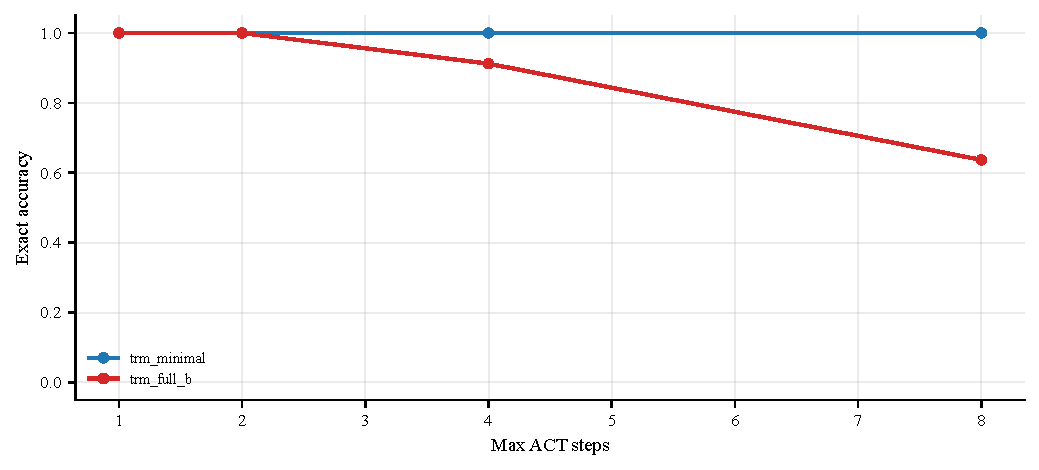
\includegraphics[width=0.95\linewidth]{figures/fig_ren_act_depth.pdf}
  \caption{ACT-depth sensitivity (Ren fixed-point stress test).}
  \label{fig:ren_act}
\end{figure}

\begin{figure}[h]
  \centering
  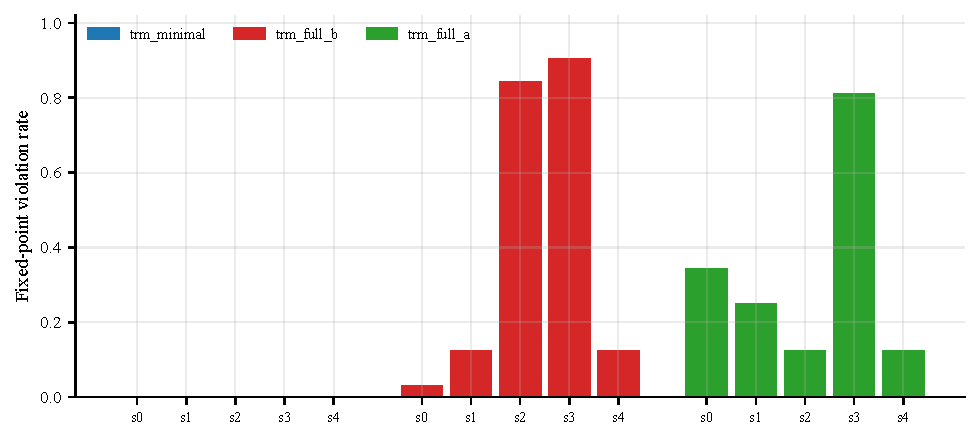
\includegraphics[width=0.7\linewidth]{figures/fig_ren_fp_violation.pdf}
  \caption{Fixed-point violation rate per seed/checkpoint: full TRM corrupts
  previously correct outputs on later ACT steps (Ren guessing), whereas minimal
  TRM is near zero (Nanda cleanup, not guessing).}
  \label{fig:ren_fp}
\end{figure}

\begin{figure}[h]
  \centering
  
\includegraphics[width=0.6\linewidth]{figures/fig_latent_pca_trajectory.pdf}
  \caption{Latent PCA across ACT steps (full TRM representative seed).}
  \label{fig:pca_ren}
\end{figure}

\begin{figure}[h]
  \centering
  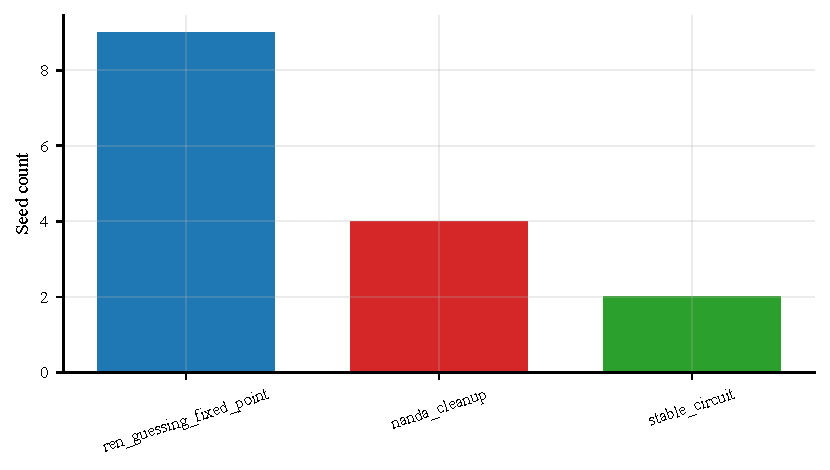
\includegraphics[width=0.7\linewidth]{figures/fig_ren_mechanism_summary.pdf}
  \caption{Per-seed post-grokking mechanism classification.}
  \label{fig:ren_mech}
\end{figure}

\begin{table}[h]
  \centering
  \caption{Post-grokking mechanism classification (Ren + Nanda probes).}
  \label{tab:ren_mechanism}
  \begin{tabular}{llll}
    \toprule
    Model & Seed & Primary mechanism & Ren applies? \\
    \midrule
    trm\_full\_a & seed\_0 & ren\_guessing\_fixed\_point & Yes \\
    trm\_full\_a & seed\_1 & ren\_guessing\_fixed\_point & Yes \\
    trm\_full\_a & seed\_2 & ren\_guessing\_fixed\_point & Yes \\
    trm\_full\_a & seed\_3 & ren\_guessing\_fixed\_point & Yes \\
    trm\_full\_a & seed\_4 & ren\_guessing\_fixed\_point & Yes \\
    trm\_full\_b & seed\_0 & nanda\_cleanup & Yes \\
    trm\_full\_b & seed\_1 & ren\_guessing\_fixed\_point & Yes \\
    trm\_full\_b & seed\_2 & ren\_guessing\_fixed\_point & Yes \\
    trm\_full\_b & seed\_3 & ren\_guessing\_fixed\_point & Yes \\
    trm\_full\_b & seed\_4 & ren\_guessing\_fixed\_point & Yes \\
    trm\_minimal & seed\_0 & stable\_circuit & Null \\
    trm\_minimal & seed\_1 & stable\_circuit & Null \\
    trm\_minimal & seed\_2 & nanda\_cleanup & Null \\
    trm\_minimal & seed\_3 & nanda\_cleanup & Null \\
    trm\_minimal & seed\_4 & nanda\_cleanup & Null \\
    \bottomrule
  \end{tabular}
\end{table}

